% =====================================================================
% SUPPLEMENTARY NOTE 6 — label transfer, and the failure it cannot report.
%
% SOURCES. x1_validation.csv for the two cross-study rows; everything else
% recomputed by figures/scripts/supp_figures.py from the shipped transfer
% file, Outputs/cells/p1_dab168_kl1/cell_family_transferred.csv.gz, which
% carries per cell the vote fraction, the mean distance to the 25
% neighbours and the donor and study count of the neighbourhood. The
% li_2025 figures therefore come from the FINAL transfer over all 640,606
% annotated cells and differ in the third decimal from the validation run
% in EXPERIMENTS.md, which trained on a 60,000-cell-per-study sample.
% =====================================================================

\section{Label transfer, and the failure it cannot report}
\label{note:transfer}

Two of the eleven studies brought cell annotations, 640{,}606 cells from
118 donors. The other nine, 937{,}122 cells from 136 donors, brought none,
and almost every published composition claim concerns a cell type in a
cohort that did not label it. The claims axis therefore begins by giving
every unlabelled cell a family, and this note is the record of how, how
well, and where it fails. The failure is the useful half: it bounds which
questions the transferred labels can be asked.

\subsection{The method}

Every unlabelled cell took the family carried by the majority of its 25
nearest annotated cells in the sixteen-dimensional latent of the reported
arm. The vocabulary is the four-level cell family, stromal, epithelial,
endothelial and immune, the only one the two annotated studies share.
Because the sources are two studies and the targets are the other nine,
every transfer is across studies and across donors by construction; the 418
cells of \texttt{duempelmann\_2026} that lacked a family label are the one
within-study exception. Three quantities were kept per cell: the winning
family's share of the 25 votes, the mean distance to those neighbours, and
how many donors and studies the neighbourhood drew on
(Table~\ref{stab:transfer-nbhd}). Nothing here reads disease status.

\begin{table}[t]
\centering
\caption[The transfer's neighbourhoods]{\textbf{Properties of the
937{,}122 transferred neighbourhoods.} The last three rows are the
distances behind Supplementary Fig.~\ref{sfig:transfer-dist}.}
\label{stab:transfer-nbhd}
\small
% GENERATED by figures/scripts/supp_figures.py. Do not edit by hand.
\begin{tabular}{@{}lr@{}}
\toprule
quantity & value \\
\midrule
cells labelled by transfer & 937{,}122 \\
median vote fraction & 1.000 \\
vote unanimous across all 25 neighbours & 94.3\% \\
vote fraction below 0.6 & 0.45\% \\
neighbourhoods drawing on more than one donor & 98.8\% \\
neighbourhoods drawing on both annotated studies & 28.8\% \\
mean distance to the 25th neighbour, granulosa & 1.514 \\
mean distance to the 25th neighbour, \texttt{li\_2025} immune & 1.712 \\
mean distance to the 25th neighbour, all other transferred & 1.528 \\
\bottomrule
\end{tabular}

\end{table}

\subsection{Validation across the study barrier}

The two annotated studies are each other's only test, so each was used to
predict the other (Table~\ref{stab:transfer-val}). Accuracy is 0.9862 and
0.9845. The number that matters is balanced accuracy against the majority
baseline, because the two studies have very different compositions:
\texttt{duempelmann\_2026} is 88\% stromal and \texttt{marecko\_2024} 53\%,
so a transfer that merely inherited the source's prior would score 0.8805
on the first and collapse to 0.5252 on the second. Balanced accuracy is
0.9596 and 0.9640 in the two directions, so it does not inherit the prior.
Within-study tests holding out a third of each study's donors give 0.970
and 0.996 balanced; crossing the study barrier costs almost nothing at four
levels.

\begin{table}[t]
\centering
\caption[Transfer validation]{\textbf{Validation of the transfer.} The two
cross-study rows predict one annotated study from the other; the two
\texttt{li\_2025} rows are the out-of-tissue test, computed on the final
transfer. Balanced accuracy weights the four families equally.}
\label{stab:transfer-val}
\small
% GENERATED by figures/scripts/supp_figures.py. Do not edit by hand.
\begin{tabular}{@{}lrrr@{}}
\toprule
test & accuracy & balanced & majority baseline \\
\midrule
\texttt{marecko\_2024} $\rightarrow$ \texttt{duempelmann\_2026} & 0.9862 & 0.9596 & 0.8805 \\
\texttt{duempelmann\_2026} $\rightarrow$ \texttt{marecko\_2024} & 0.9845 & 0.9640 & 0.5252 \\
\midrule
\texttt{li\_2025} immune, out of tissue, called immune & 0.9969 & -- & -- \\
\texttt{li\_2025} granulosa, no counterpart, called stromal & 0.9874 & -- & -- \\
\bottomrule
\end{tabular}

\end{table}

\subsection{The failure: a type absent from the reference is absorbed}

\texttt{li\_2025} is follicular fluid and brought its own cell-type
column, which makes it the only out-of-tissue test available. Its 30{,}207
immune cells, neutrophils, monocytes and macrophages, T and NK cells,
dendritic cells and B cells, were called immune at 0.9969; immune identity
transfers across tissue. Its 15{,}056 granulosa cells have no counterpart
in an endometrial vocabulary, so no correct answer exists for them, and
0.9874 of them were called stromal. A family the reference does not contain
is not flagged; it is absorbed into whichever family it most resembles.

Two rejection rules were tried and neither catches it
(Tables~\ref{stab:transfer-rej} and~\ref{stab:transfer-vote},
Supplementary Figs.~\ref{sfig:transfer-dist} and~\ref{sfig:transfer-vote}).
Distance is worse than useless: granulosa cells sit closer to the reference,
at a mean distance of 1.514 to their 25th neighbour, than
\texttt{li\_2025}'s correctly called immune cells do at 1.712, so at every
distance cut the share of correct immune calls discarded is at least as
large as the share of granulosa cells rejected. Vote fraction does better
and still fails: the strictest rule, rejecting any cell whose 25 neighbours
are not unanimous, rejects 11.9\% of granulosa cells while losing 0.4\% of
the immune calls and 5.7\% of all other transferred cells, and leaves the
remaining 88\% of granulosa cells confidently stromal. The transfer cannot
tell when it is wrong, and no quantity it produces can be thresholded into
telling.

\begin{table}[t]
\centering
\caption[A distance rule does not work]{\textbf{Rejecting cells by distance
to the reference.} Share of each group discarded at each cut on the mean
distance to the 25 nearest annotated cells.}
\label{stab:transfer-rej}
\small
% GENERATED by figures/scripts/supp_figures.py. Do not edit by hand.
\begin{tabular}{@{}rrrr@{}}
\toprule
distance cut & granulosa rejected & \texttt{li\_2025} immune lost & other transferred cells lost \\
\midrule
1.5 & 46.8\% & 78.1\% & 44.5\% \\
2.0 & 6.4\% & 13.7\% & 13.5\% \\
2.5 & 0.4\% & 0.5\% & 3.5\% \\
3.0 & 0.0\% & 0.0\% & 1.0\% \\
\bottomrule
\end{tabular}

\end{table}

\begin{table}[t]
\centering
\caption[A vote rule does not work either]{\textbf{Rejecting cells by vote
fraction.} Share of each group discarded when cells below each vote share
are left unlabelled.}
\label{stab:transfer-vote}
\small
% GENERATED by figures/scripts/supp_figures.py. Do not edit by hand.
\begin{tabular}{@{}rrrr@{}}
\toprule
vote fraction & granulosa rejected & \texttt{li\_2025} immune lost & other transferred cells lost \\
\midrule
$<$ 1.0 & 11.9\% & 0.4\% & 5.7\% \\
$<$ 0.9 & 3.1\% & 0.2\% & 2.9\% \\
$<$ 0.8 & 1.4\% & 0.1\% & 1.6\% \\
$<$ 0.6 & 0.3\% & 0.0\% & 0.5\% \\
\bottomrule
\end{tabular}

\end{table}

\begin{figure}[t]
\centering
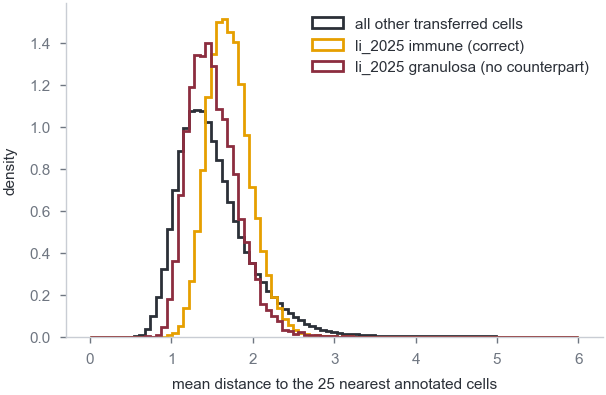
\includegraphics[width=.65\textwidth]{figures/transfer_distance_by_group.png}
\caption[Distance to the reference, by group]{\textbf{Distribution of the
mean distance to the 25 nearest annotated cells}, for granulosa cells, for
\texttt{li\_2025}'s immune cells and for every other transferred cell. The
cells with no correct answer are not the distant ones.}
\label{sfig:transfer-dist}
\end{figure}

\begin{figure}[t]
\centering
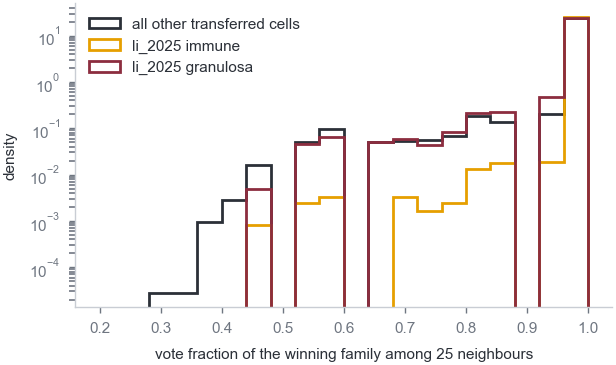
\includegraphics[width=.65\textwidth]{figures/transfer_vote_by_group.png}
\caption[Vote fraction, by group]{\textbf{Distribution of the winning
family's vote share}, same three groups, log density.}
\label{sfig:transfer-vote}
\end{figure}

\subsection{What the transferred labels can and cannot be asked}

Asking what family a cell belongs to is sound wherever the cell's type
exists in an endometrial reference. Counting families in a tissue that may
contain types the reference lacks is not, because the unknowns are added
silently to whichever family absorbs them. The tissues that condition is
ovary, peritoneum, myometrium and follicular fluid, which is where the
ectopic and adenomyosis donors are, and it is why the lesion composition
test in Supplementary Note~\ref{note:claims} carries a warning that the
endometrium tests do not. The absorption error there runs against the one
result it could affect: mesothelial cells line the peritoneum, have no
endometrial counterpart and would be pushed into the epithelial or stromal
family, which would raise the epithelial share in lesions, and that share
is lower.

Table~\ref{stab:transfer-comp} and Supplementary Fig.~\ref{sfig:transfer-comp}
give the transferred composition of each study. Two rows are informative
about the deposits rather than the model. \texttt{garcia\_alonso\_2021\_b}
comes out 99.9\% epithelial, which identifies it as an epithelium-sorted
sample rather than whole tissue, and \texttt{li\_2025}'s 66.8\% immune and
33.1\% stromal is the granulosa absorption as the validation predicted it.
\texttt{shih\_2022} at 78.2\% immune is plausible, since menstrual effluent
is blood-rich.

\begin{table}[t]
\centering
\caption[Transferred composition by study]{\textbf{Transferred cell-family
composition of each study.} \texttt{duempelmann\_2026}'s row is the 418
cells of that study that lacked a label.}
\label{stab:transfer-comp}
\small
% GENERATED by figures/scripts/supp_figures.py. Do not edit by hand.
\begin{tabular}{@{}lrrrrr@{}}
\toprule
study & cells transferred & stromal \% & epithelial \% & endothelial \% & immune \% \\
\midrule
\texttt{duempelmann\_2026} & 418 & 44.5 & 32.1 & 1.0 & 22.5 \\
\texttt{ferrero\_2024} & 15{,}872 & 56.7 & 2.7 & 13.9 & 26.7 \\
\texttt{fonseca\_2023} & 386{,}560 & 62.7 & 1.1 & 6.0 & 30.1 \\
\texttt{garcia\_alonso\_2021\_a} & 100{,}096 & 54.4 & 36.0 & 7.4 & 2.2 \\
\texttt{garcia\_alonso\_2021\_b} & 10{,}240 & 0.0 & 99.9 & 0.0 & 0.0 \\
\texttt{li\_2025} & 45{,}312 & 33.1 & 0.0 & 0.0 & 66.8 \\
\texttt{lin\_2023} & 140{,}032 & 47.0 & 27.5 & 6.5 & 19.0 \\
\texttt{shih\_2022} & 74{,}496 & 14.9 & 6.6 & 0.3 & 78.2 \\
\texttt{tan\_2022} & 114{,}944 & 41.4 & 16.7 & 10.2 & 31.7 \\
\texttt{wang\_2022} & 49{,}152 & 58.0 & 4.3 & 31.3 & 6.4 \\
\bottomrule
\end{tabular}

\end{table}

\begin{figure}[t]
\centering
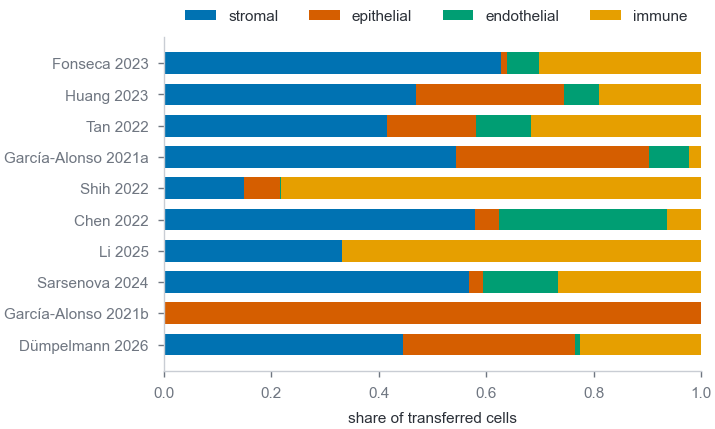
\includegraphics[width=.65\textwidth]{figures/transfer_composition_by_study.png}
\caption[Transferred composition, drawn]{\textbf{Table~\ref{stab:transfer-comp}
drawn}, studies ordered by cells transferred.}
\label{sfig:transfer-comp}
\end{figure}
